%%%%%%%%%%%%%%%%%%%%%%%%%%%%%%%%%%%%%%%%%%%%%%%%%%%%%%%%%%%%%%%%%%%%%%%%%%%%%%%%
%	Latex Notes Template
%	Zach Neveu
%	zachary.neveu@gmail.com
%%%%%%%%%%%%%%%%%%%%%%%%%%%%%%%%%%%%%%%%%%%%%%%%%%%%%%%%%%%%%%%%%%%%%%%%%%%%%%%%

% Geometry, font
\documentclass[12pt, letter]{article}
\usepackage[margin=0.8in]{geometry}
\usepackage[T1]{fontenc}
\usepackage{fourier}
\usepackage{titling}
\setlength{\droptitle}{-5em} 
\usepackage[parfill]{parskip}
\usepackage{graphicx}
\usepackage{hyperref}

% Math stuff
\usepackage{amssymb}
\usepackage{amsmath}
\usepackage{bm}

%acronyms
\usepackage{acronym}


% Code Highlighting
\usepackage{minted}
\usemintedstyle{solarizedlight}

\author{Zach Neveu}
\title{ Project 2 Description }

\begin{document}
\maketitle

The basic idea of my project was to create a looper that incorporates 4 voices of pitch shift without time stretching. The idea for this setup is to be able to create harmonies from recorded loops, allowing for a huge space of potential ways to re-imagine a melody. The majority of my time was spent figuring out pure data basics, and understanding the concepts behind tape-wheel style pitch shifting.

\subsection*{Circuit}
The circuit diagram is shown in fig. \ref{fig:circuit}. The basic components are quite simple: 4 potentiometers connected to analog inputs, and one push button connected to a digital input.

\begin{figure}[h]
	\centering
	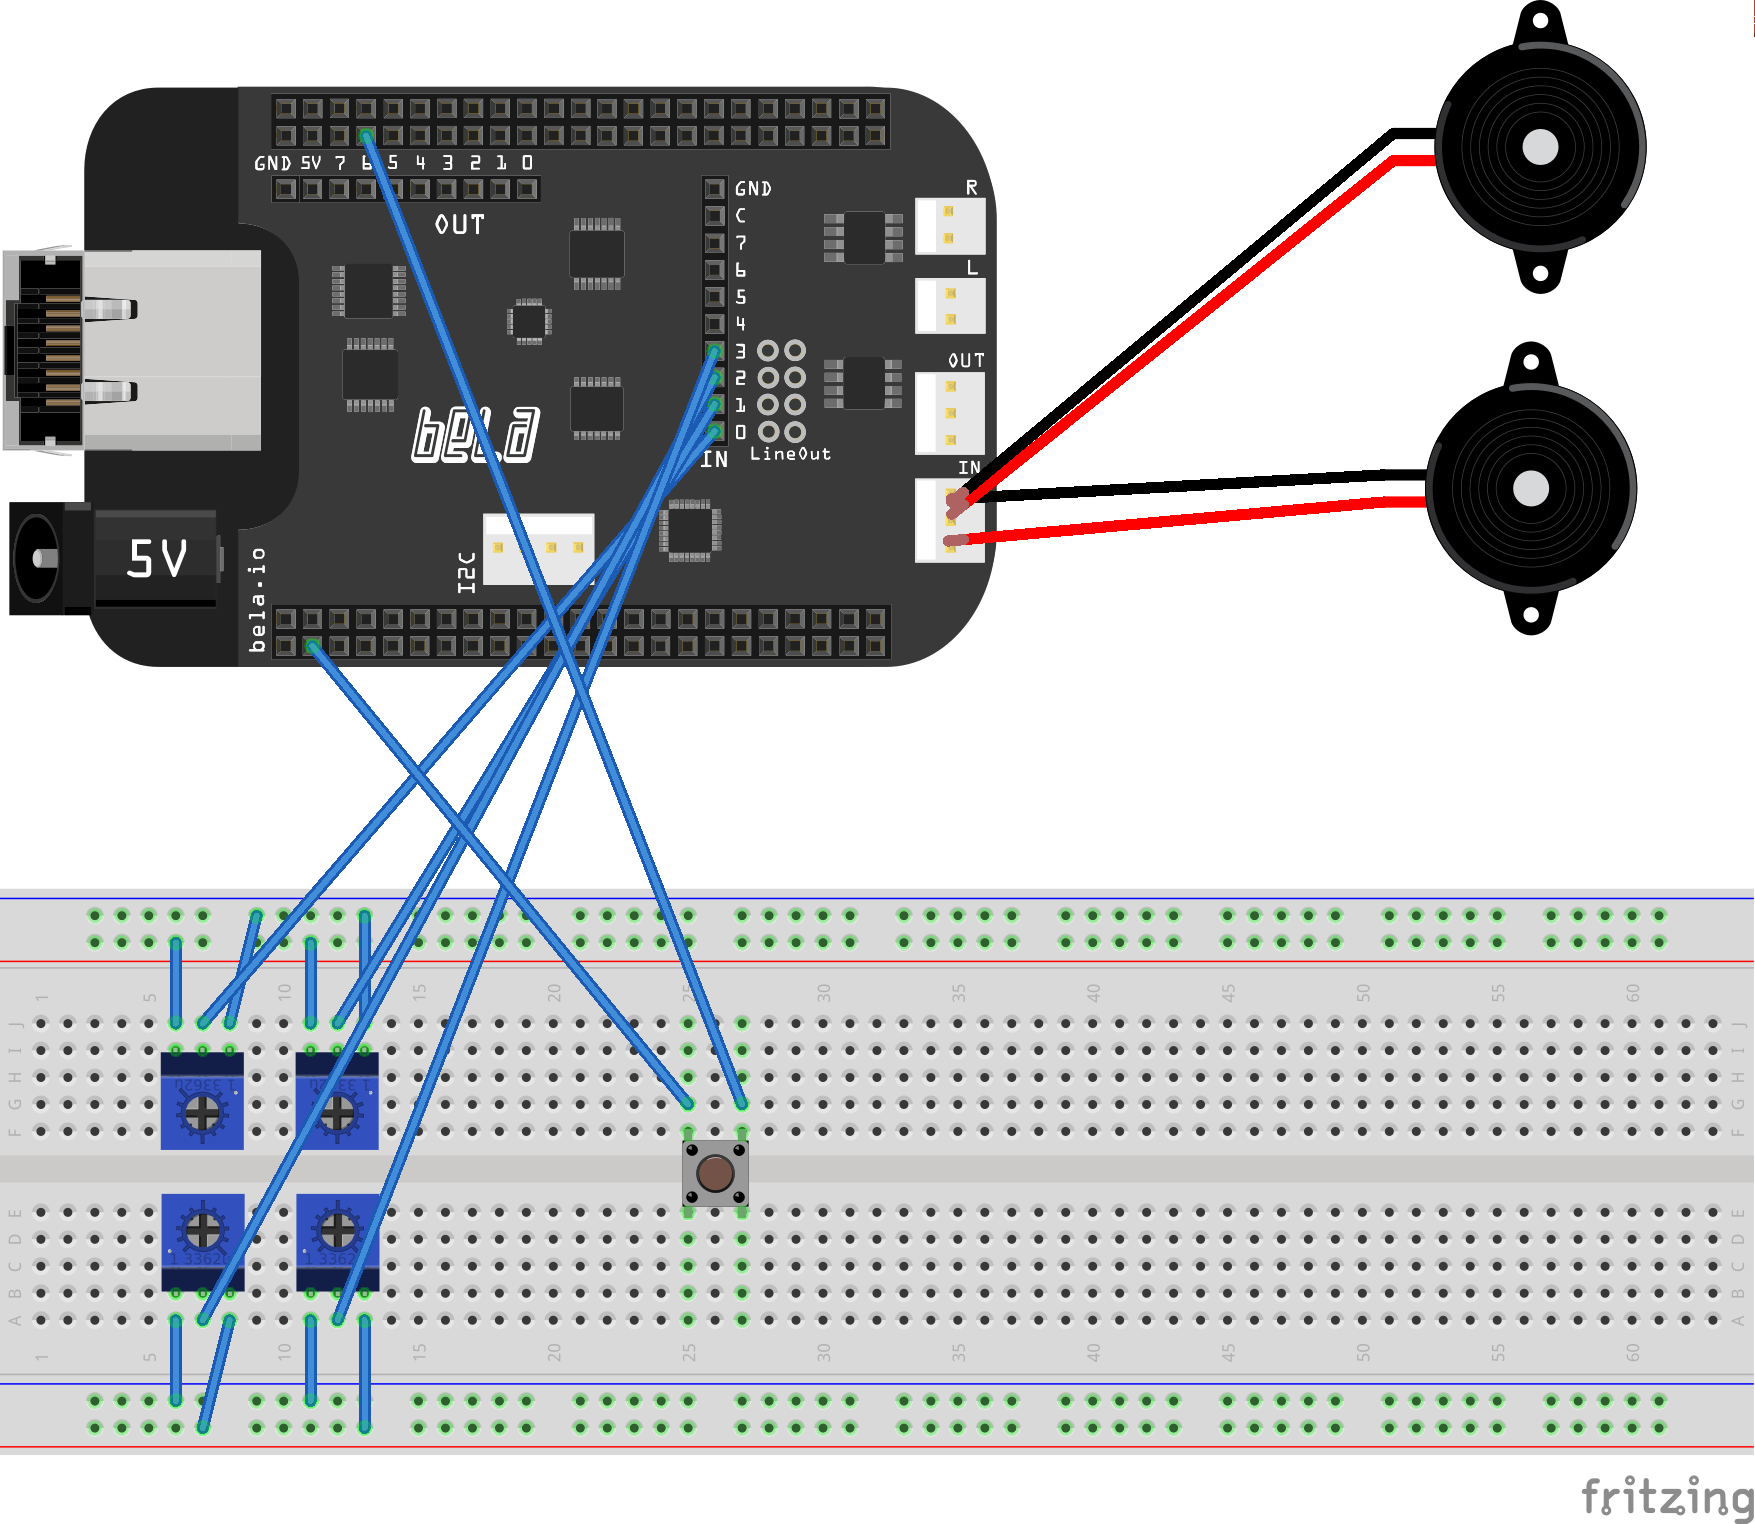
\includegraphics[width=0.8\textwidth]{../p2_schematic.png}
	\caption{Fritzing Breadboard Model of Circuit}
	\label{fig:circuit}
\end{figure}

\begin{figure}[h]
	\centering
	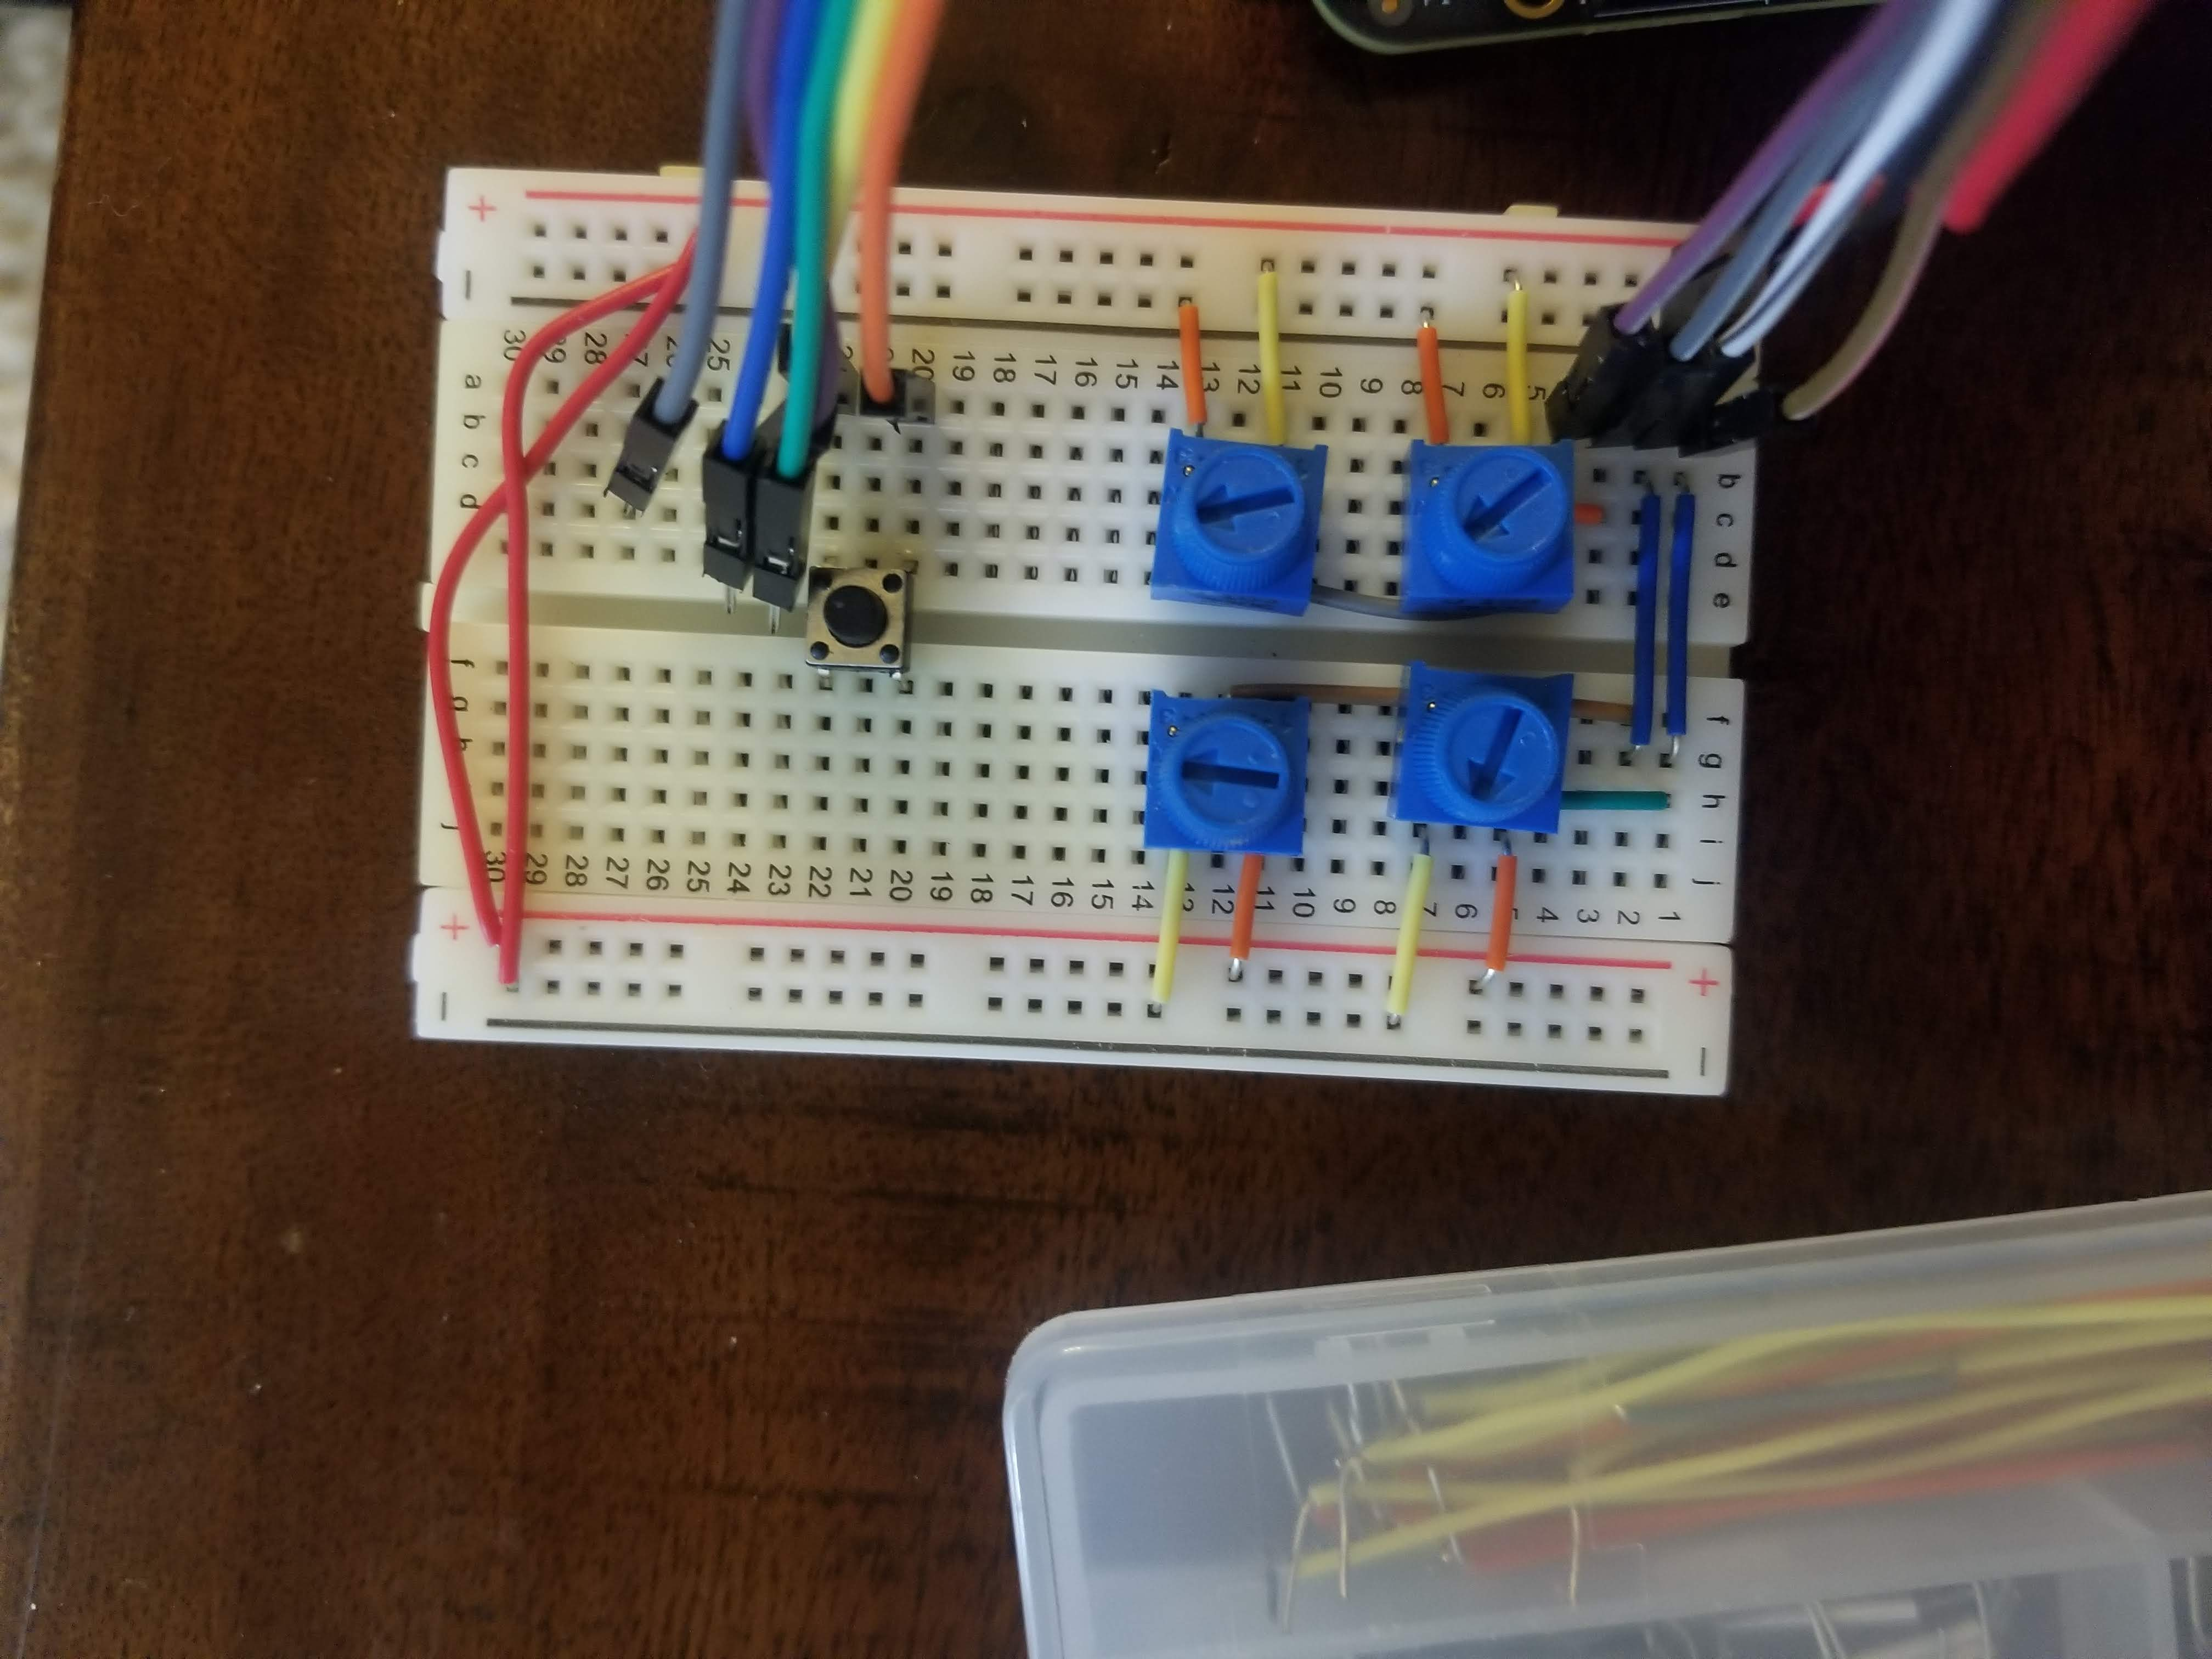
\includegraphics[width=0.8\textwidth]{../p2_circuit.jpg}
	\caption{Picture of Breadboard Circuit}
	\label{fig:-p2_circuit-jpg}
\end{figure}

\end{document}
